% The preprint version of the manuscript: the same sections as main.tex, in a plain article layout that does not
% depend on the template of any venue. It names no venue. build-preprint.sh defines \authorfile, a file kept outside
% the repository that defines \ppauthor, \ppaffiliation, \ppemail and \pporcid; see BUILD.md.
\documentclass[10pt,twocolumn,letterpaper]{article}
\usepackage[margin=0.75in,columnsep=0.33in]{geometry}
\usepackage[T1]{fontenc}
\usepackage{newtxtext,newtxmath}
\usepackage{microtype}
\usepackage{amsmath}
\usepackage{booktabs}
\usepackage{array}
\usepackage{graphicx}
\usepackage[numbers,sort&compress]{natbib}
\usepackage{pgfplots}
\pgfplotsset{compat=1.18}
\usepackage[hidelinks]{hyperref}
\usepackage{xurl}
\usepackage[font=small,labelfont=bf]{caption}

% Rows of the result tables, generated by make_tables.py; the primitive input works inside a tabular.
\makeatletter
\newcommand{\tabinput}[1]{\@@input #1 }
\makeatother

% The statements that the submission template sets as unnumbered sections.
\newenvironment{ethics}{\section*{Ethical Considerations}}{}
\newenvironment{openscience}{\section*{Open Science}}{}
\newenvironment{ai}{\section*{AI Use}}{}

\ifdefined\authorfile
\input{\authorfile}
\else
\errmessage{preprint.tex needs the author file; build it with build-preprint.sh}
\fi

\title{Hiding the Text, Keeping the Process: Matching Processed Keystroke Logs to Texts Held by Others}
\author{\ppauthor\\[2pt]
  \normalsize \ppaffiliation\\
  \normalsize \href{mailto:\ppemail}{\ppemail} \quad ORCID \href{https://orcid.org/\pporcid}{\pporcid}}
\date{Preprint, \today}

\begin{document}

\twocolumn[
  \begin{@twocolumnfalse}
    \maketitle
    \begin{center}
      \begin{minipage}{0.85\textwidth}
        \small
        \textbf{Abstract.}
        % The abstract, shared by main.tex (the submission) and preprint.tex (the preprint).
  Keystroke logs record how a text was written. One public release of essay logs masked every letter and digit, with
  the stated goal of preventing reproduction of the essays, while the essays themselves had been collected and scored
  and remained with others. For the writers' privacy, a log linked to its text tells the holder of the text how its
  writer wrote it, with the pauses, the revisions and any score, and in a classroom this would concern a named student.
  We ask how far each form of processing keeps a keystroke log apart from its text, which is how we read that goal,
  against a party that holds candidate texts, and what each form costs the process measures of writing research. In a preregistered evaluation on
  500 writers sampled from a public corpus of 4,992 essays with their logs, attackers that know the processing chose
  the true text among $N$ candidates on the same prompt. Against the masking, an attacker that rebuilds the final
  draft chose the true essay among 1,000 for every log, 98 percentage points above an attacker that uses only the
  total length. Keeping only the categories of the pressed keys and their press times still left 86.7\% (95\%
  interval 83.5 to 89.5). Forms that release less traded matching for the process measures: suppressing a quarter of
  the presses left 14.3\% with a median correlation of 0.81 with the unprocessed measures, and only segment values
  coarsened to four or more brought the full-text attackers, with their main penalty, within four times chance at
  $N = 1{,}000$, computing no measure. Exploratory attackers fixed after these results, with a lighter penalty or
  aligning parts of a log anywhere in a text, raised the quarter suppression to 62.3\% and segment values coarsened to
  four to 48.2\%, and no form stayed within four times chance. On
  Japanese translation logs typed with an input method, matching without any string chose the true translation in
  51.6\% of logs among 12 or 13 candidates, against 7.9\% by chance. The results describe the attackers tried and are not bounds on the risk.


        \smallskip
        \textbf{Keywords:} keystroke logging, data release, de-identification, matching attack, writing process
      \end{minipage}
    \end{center}
    \bigskip
  \end{@twocolumnfalse}
]
\begingroup
\renewcommand{\thefootnote}{}
\footnotetext{This work is licensed under the Creative Commons Attribution 4.0 International License
(\url{https://creativecommons.org/licenses/by/4.0/}).}
\endgroup

\section{Introduction}
\label{sec:introduction}

% Follows the plan of the first page in outline.md; the first page must state how the work is relevant to real-world
% privacy. The last three paragraphs were written after the main results (24 October 2026).

Keystroke logs record how a text was written: every press and release, the pauses between them, the revisions and the
movements of the cursor. Writing research uses them to study the process of writing, and public corpora release logs
together with their texts and scores~\cite{tian2025klicke}. A~log also carries the text it produced, so a release
that is meant to keep the text apart from the process has to hide the text. One public release did this by masking
letters and digits:
the logs of a Kaggle competition on writing quality replaced every letter and digit by \texttt{q}, with the stated goal
``to prevent reproduction of the essay text''~\cite{kaggle2023lwp}. The lengths of words, the punctuation, the times
and the cursor positions remained, and the winning solution rebuilt the masked essays from the logs and used their
word and sentence lengths to predict their scores~\cite{inubushi2024first}.

The texts of such essays do not disappear when the logs are released. They were collected and scored, so they are held by
those who collected and scored them, and texts on the same prompts can be public; in a classroom, a teacher holds the
texts of a class. The authors of a public corpus, KLiCKe~\cite{tian2025klicke}, told us that the competition data were
drawn from that corpus before it was released with its texts; we did not check whether the released corpus contains the hidden essays
(Section~\ref{sec:threat-model:settings}). A party
who holds candidate texts does not need a labelled sample of a writer's keystrokes, which earlier work on releasing
keystroke data assumed an attacker would need~\cite{edwards2023csedm}; it can compare what the processed log leaves with
each text. This paper asks how far processing keeps logs apart from their texts against such a party, which is how we read the
stated goal, and what each form of processing costs research.

We answer this for one processed log against $N$ candidate texts on the same prompt, in a closed world, with $N =
10$, $100$ and $1{,}000$, on a public corpus whose texts are known (KLiCKe). The forms are the masking used in the
competition and alternatives that release less: key categories, merged separators, rounded times, segment values
alone and random suppression of presses. The attackers know the processing and range from one that uses only the
total length to one that rebuilds the final draft and one that scores the press intervals. For each form we report
the strongest attacker's accuracy, as a multiple of $1/N$ and as a gain over the total length, and how far ten
standard process measures of writing research can still be computed; the same kind of matching is also run on
Japanese translation logs typed with an input method. The study was preregistered before any data were acquired.

The main harm we consider is the link between a processed log and its text for a party that holds the text: the times,
the revisions and any released score of the log are then linked to that text. Where the writer of a text is known, as
in a class or for an essay its writer has published, the log would also be linked to a named person; we know of no
release in which this has happened and state it only as a consequence (Section~\ref{sec:threat-model}).

Against the attackers tried, the masking kept no log apart from its text: an attacker that rebuilds the final draft,
as the winning solution of the competition did, chose the true essay among 1,000 for every log (C1,
Section~\ref{sec:results:masking}). Forms that release less lowered matching only at a cost to the process measures:
keeping the key categories still left 86.7\% at $N = 1{,}000$, every form that kept the measures close to their
unprocessed values (a median correlation of 0.84 or more) left 70\% or more, and the forms that brought matching near the total length kept them at a
median correlation of at most 0.70 or not at all (C2, Sections~\ref{sec:results:forms} and~\ref{sec:results:utility}). We frame a threat in which the
auxiliary information is the text, held outside the release, and give the settings in which it arises (C3,
Section~\ref{sec:threat-model}). The results describe the attackers tried; they are not bounds on the risk.

\section{Background and related work}
\label{sec:related}

To be written.

\section{Threat model}
\label{sec:threat-model}

This section describes how keystroke logs of writing are released (\S\ref{sec:threat-model:releases}), the kind of
auxiliary information that this study considers (\S\ref{sec:threat-model:auxiliary}) and who holds it
(\S\ref{sec:threat-model:settings}). It then states the attacker (\S\ref{sec:threat-model:attacker}) and the direction
in which the assumptions bias the results (\S\ref{sec:threat-model:bias}). The attacker's knowledge, the candidate sets
and the list of attackers were fixed in the preregistration of this study before any data were acquired; this section
motivates them and does not change them.

\subsection{Releases of keystroke logs}
\label{sec:threat-model:releases}

\paragraph{Logs are released with the text hidden.}
Keystroke logs of writing are released to support research on the writing process, and a release may hide the text
and keep the rest of the log. The Kaggle competition ``Linking Writing Processes to Writing Quality'' released logs of
argumentative essays in which, in the words of its data description, ``to prevent reproduction of the essay text, all
alphanumeric character inputs have been replaced with the `anonymous' character q;\ punctuation and other special
characters have not been anonymized''~\cite{kaggle2023lwp}. The released columns include the press and release times,
the activity, the text change, the cursor position and the word count. This is the release that motivates the study:
the text is hidden, and every letter and digit is still present as a press.

\paragraph{The lengths that remain are used.}
Masking each letter and digit keeps the length of every word. The winning solution of the competition began by
rebuilding the essay from the masked log (``the first thing I did in this competition is to reconstruct sentences from
keyboard activities'') and used statistics of the rebuilt text, such as words per sentence and word length, to predict
the score~\cite{inubushi2024first}. The structure that makes a masked log useful for research on writing is also the
structure that a party holding candidate texts can compare with those texts.

\paragraph{Other masking keeps lengths too.}
Two public datasets of keystrokes in an introductory programming course mask the characters of identifying text, such
as a student's name, with the character \texttt{@}; a~function \texttt{even()} in which the name ``Eve'' was masked
becomes \texttt{@@@n()}~\cite{edwards2023csedm}. This release hides names, not the program, so it is not an instance of
the threat studied here; it shows that masking one character for one character is a common choice, and with it the
lengths of the masked strings remain. The times of the events are not processed in this release.

\paragraph{Parts of logs.}
A log may also be shared or analysed only in part. The evaluation therefore covers windows of a log as well as full
logs (Section~\ref{sec:protocol}).

\subsection{Auxiliary information other than labelled keystrokes}
\label{sec:threat-model:auxiliary}

Earlier work on releasing keystroke data considered an attacker who holds a labelled sample of the same person's
keystrokes. Keystroke latencies link students across samples, and rounding the latencies in typing profiles reduced
identification~\cite{leinonen2017preventing}. The paper that released the programming datasets answers the risk of
identification by timing in the same terms: ``all of these identification techniques require a labeled sample, which
the regulatory definition of identifiability assumes is not available'', and ``the data is deidentified only as long
as there is no other labeled sample of a student's keystrokes''~\cite{edwards2023csedm}. A survey of anonymisation for
behavioural biometric data notes that ``most anonymization techniques are only evaluated rudimentarily with the
assumption of a weak attacker''~\cite{hanisch2021survey}.

This study considers a different kind of auxiliary information: the texts. Records in a release can be linked to
outside information that the releasing party did not anticipate~\cite{narayanan2008robust}, and for logs of writing the
most direct such information is the text that was written. A log matched to a text whose writer is known would, from
then on, also be a labelled sample of that writer's keystrokes.

\subsection{Who holds the texts}
\label{sec:threat-model:settings}

A hidden text can be matched only if it exists somewhere outside the release. Table~\ref{tab:settings} lists the
settings we consider. They differ in what the holder has, in the direction of the search and in whether the true text
is always among the candidates (the closed world assumed by the evaluation).

\begin{table*}
  \caption{Settings in which texts are held outside a release of processed logs.}
  \label{tab:settings}
  \small
  \begin{tabular}{>{\raggedright\arraybackslash}p{0.15\linewidth}>{\raggedright\arraybackslash}p{0.19\linewidth}>{\raggedright\arraybackslash}p{0.12\linewidth}>{\raggedright\arraybackslash}p{0.19\linewidth}>{\raggedright\arraybackslash}p{0.21\linewidth}}
    \toprule
    Setting & Holder has & Direction & Closed world holds when & Newly learned by matching \\
    \midrule
    Public corpus on the same prompts & Texts of a public corpus collected in the same way & One log, many texts &
      The hidden essays are in the corpus & The hidden text, and the score and process columns of its log \\
    Classroom & The texts and names of the students of a class or course & One log, many texts & The release consists
      of that class & The writing process, given for research, of a named student \\
    Published essay & One text and its writer, found in a class or online & One text, many logs & Rarely: the log need
      not be in the release (open world) & The writing process and score of a known writer \\
    \bottomrule
  \end{tabular}
\end{table*}

\paragraph{A public corpus on the same prompts.}
The KLiCKe corpus was collected on Amazon Mechanical Turk in 2022 and released together with its keystroke logs and
human scores: 4,992 argumentative essays on four prompts derived from the SAT, each written in 30
minutes~\cite{tian2025klicke}. Because its texts are public, its logs need no protection of the text; it is the
data on which we evaluate the processing. The description of the procedure of the competition data names the same
platform, the same kind of prompts and the same sequence of tasks~\cite{kaggle2023lwp}. A public set of about a
thousand essays per prompt is therefore the kind of candidate set that a text-hidden release on the same prompts would
face. The closed world holds only if the hidden essays are among the public ones. We did not examine whether the two
releases share essays, for ethical reasons (see the ethical considerations).

\paragraph{Classrooms.}
Teachers and course staff hold the texts submitted by their students, with names. The programming datasets above were
collected in a course~\cite{edwards2023csedm}, and writing tools now keep the text and the writing process of students
in one product and offer a replay of the process to instructors~\cite{grammarly2026authorship,turnitin2026clarity}.
We know of no release of logs from such tools for research. If a release contained the logs of one class with the
text processed, its teacher would hold every candidate; if the release spans many classes, the teacher holds the
candidates for only part of it, and the closed world does not hold.

\paragraph{A published essay.}
An essay may be published by its writer, in a class or online. A party who finds it holds one text and searches a
release for its log. The search runs in the other direction, and the log may not be in the release at all. The
evaluation does not run this direction, and its closed-world accuracy is only a guide in this setting: with many logs
to search and a true log that may be absent, false matches are expected to be more frequent.

\paragraph{Translation.}
In research on the translation process, translations of the same source text by other translators are held by the
researchers who collected them. The Japanese translation logs evaluated in this study use these translations as
candidates (Section~\ref{sec:results}).

\subsection{Attacker}
\label{sec:threat-model:attacker}

\paragraph{Knowledge.}
The attacker holds one processed log and $N$ candidate texts that include the true text, all written on the same
prompt. The attacker knows the processing procedure, following Kerckhoffs's principle~\cite{kerckhoffs1883}. The
attacker may train on public data of the same kind, that is, logs before processing paired with their texts; in this
study these are the writers of the prompts that are not being evaluated, and their texts are never candidates. Beyond
the processed log and the candidates, the attacker does not use the writer's earlier texts, text generated by language
models, or links across several releases (such as several logs of the same writer). In the taxonomy of Wagner and
Eckhoff~\cite{wagner2018metrics}, the attacker is passive, external (it observes the release from outside the
releasing party) and static, and has prior knowledge (the candidate set and the training data). One attacker in this
study, the public KeyTAR model~\cite{qiu2026keytar}, contains a public language model; it is reported as a reference
outside this threat model.

\paragraph{Goals and harms.}
The main harm is (b): linking a log and its other columns (times, pauses, the revision process, pasting, the score)
to a text and, where the writer of the text is known, to the writer. In the classroom and published-essay settings,
this ties a record that a writer gave for research to a named person. A secondary harm is (a): learning which text a
processed log hides, which defeats the purpose of the processing even when that text is public elsewhere. Both rest on
the link between a log and its text, which is what this study measures; the study does not identify writers. Because
the protection given by a processing step may differ between writers, the distribution of accuracy per writer is
reported as well as the mean.

\paragraph{Size of the candidate set.}
We use $N = 10$, $100$ and $1{,}000$. The value $1{,}000$ is the size of a public corpus on one prompt; $10$ and
$100$ are illustrative sizes of a class or a list of submissions and of a year or a course. $N$ gives only the number
of candidates. The decoys are drawn uniformly from writers on the same prompt, who need not be as similar to one another
as the members of one class.

\subsection{Assumptions and the direction of bias}
\label{sec:threat-model:bias}

Some assumptions favour the attacker: the true text is always among the candidates (the closed world, examined
otherwise only as a diagnostic), the attacker trains on data collected in the same way as the evaluated logs, and in
windows the attacker knows where the window starts and ends. Others limit it: the attackers do not use language models,
the writer's earlier texts or several releases, because the study measures what the processed columns themselves leave.
The results therefore describe the attackers tried here, under these assumptions. They give no proof of safety and no
upper bound on the risk of matching; a processing step that defeats these attackers may not defeat a stronger one.

Under this threat model a releasing party chooses which columns to keep, how coarsely to give times and lengths, and
whether to release full logs or parts of them. The results are material for that choice; they do not recommend a
form.

\section{Data and release forms}
\label{sec:data}

To be written.

\section{Attackers}
\label{sec:attackers}

% What this part is meant to establish and what is measured. What was found and why it matters are written in
% Section 7 after the results.
The attackers are meant to show what a party that holds candidate texts and knows the processing can do with what a
form leaves; what is measured is the accuracy of each attacker, and of the strongest one, on each form
(Section~\ref{sec:protocol}). Each attacker compares what a form leaves of a log with each candidate text and chooses
the candidate that fits best. Most of them compare sequences of segment values, which roughly correspond to word
lengths (\S\ref{sec:attackers:segments}), through a common alignment (\S\ref{sec:attackers:alignment}). All attackers
know the processing, and no attacker uses a column that its form does not release.

\subsection{Segments}
\label{sec:attackers:segments}

\paragraph{Texts.}
In a text, a word is a run of letters and digits, and its segment value is the number of letters and digits in it;
other characters separate words.

\paragraph{Logs.}
In a log, segments are counted from the key categories alone. A letter or digit press adds 1, a BackSpace press
subtracts 1, and a space, punctuation or Enter press closes the segment. If the next press after a Control or Meta
press, other than a modifier, is a letter or digit, it is a shortcut and is neither counted nor a separator; whether
Control is still held cannot be read, because the corpus gives modifier presses an action time of zero. Navigation,
other modifiers, mouse, Delete and other presses are neither counted nor separators, and a trailing open segment is
kept if it contains a counted press. Deletion of a selection, paste and replacement cannot be seen in the categories
and are counted by this rule as they are, so the value of a segment can differ from the length of the word it became.

\paragraph{Error of the rule.}
The checks after acquisition compared the value of each segment with the number of its counted characters that
survive in the final draft, obtained by replaying the unprocessed log. Of the 2,381,444 segments with at least one
counted press, the two values agree for 77.1\%; the share of agreeing segments per writer has a median of 0.80 (10th
percentile 0.62, 90th percentile 0.92). Empty segments, which arise for example after a comma followed by a space,
agree by construction and are not included in these shares. The error is reported with the tables, and the rule was
not changed; cases that the rule misses are described in Appendix~\ref{app:checks}.

\subsection{Alignment}
\label{sec:attackers:alignment}

Attackers A1, A1', A2 and A3 align a sequence of record segments with a sequence of text segments by dynamic
programming. A group maps $p$ record segments to $q$ text segments, with $(p, q)$ one of $(1,1)$, $(2,1)$, $(1,2)$,
$(3,1)$ and $(1,3)$, which absorbs a separator that was typed but not kept or kept but not typed. The cost of a group
is
\[
  \Bigl|\sum \text{record values} - \sum \text{text values}\Bigr| + \lambda\,(p - 1 + q - 1),
\]
with $\lambda = 8$, a value fixed in earlier prototypes and not tuned on these data; $\lambda = 4$ and $16$ are reported
as a secondary analysis. Among paths of equal cost, the group listed first is chosen, and where the end can be chosen, the earlier position in the
text. In full-text matching both
sequences are used to their ends; in window matching the whole window is used and the text may end early. Under
suppression (R7), dropping a separator press merges record segments, so the groups are extended to $(p', 1)$ and
$(1, q)$ with $p', q$ up to $\lceil 3/(1-p) \rceil$, that is 4 for $p = 0.1$ and $0.25$ and 6 for $p = 0.5$; the
cost is the same. This alignment ignores the binomial variation of suppression and is not a likelihood. A candidate
with no path has infinite cost and is never chosen; if every candidate has infinite cost, all candidates tie. The
numbers of such cases are reported.

\subsection{Attackers}
\label{sec:attackers:list}

Table~\ref{tab:attackers} lists the attackers and the forms on which each is run. Attackers A2-b and A3 are trained on
the unprocessed logs and texts of all writers of the two prompts not being evaluated, with the evaluated form applied to
the training logs. The strongest attacker of a form is the best of the adaptive attackers (A0 to A3, including A1$'$ and A2-b) on that
form
(\S\ref{sec:protocol:quantities}).

\begin{table*}
  \caption{Attackers. A0 to A3 are within the threat model and adapt to the processing; A4 is a reference outside the
  threat model.}
  \label{tab:attackers}
  \small
  \begin{tabular}{>{\raggedright\arraybackslash}p{0.16\linewidth}>{\raggedright\arraybackslash}p{0.17\linewidth}>{\raggedright\arraybackslash}p{0.58\linewidth}}
    \toprule
    Attacker & Forms & What it compares \\
    \midrule
    A0 Total length & All & Letter and digit presses minus BackSpace presses in the log (R3-u: ``char'' presses
      minus BackSpace; R7: the remaining presses scaled by $1/(1-p)$), against the number of letters and digits in the
      candidate (R3-u: all characters); in R4, the sum of the released values against the sum of $\lfloor v/w
      \rfloor$ over the candidate's segments \\
    A1 Final-draft lengths & R0, R1, R2, R5, R6 & The final draft is rebuilt from the text change and the position (R2:
      the categories and the position), as in the winning solution of the competition~\cite{inubushi2024first}, and
      its word lengths are aligned with the candidate's \\
    A1$'$ Editor replay & R3, R3-t, R7 & The category column is replayed as an editor, and the word lengths of the
      replayed draft are aligned with the candidate's (R7: candidate lengths scaled by $1-p$) \\
    A2 Segment alignment & R2, R3, R3-t, R4, R7 & The record segments are aligned with the candidate's segments (R4:
      both as $\lfloor v/w \rfloor$; R7: candidate values scaled by $1-p$) \\
    A2-b Boundary estimation & R3-u & A logistic regression predicts which ``char'' presses are separators from the
      intervals around them; the predicted segments are aligned as in A2 \\
    A3 Timing & R0, R1, R2, R3, R3-t, R3-u, R5, R6, R7 & The likelihood of the press intervals under the character
      pairs of the candidate, on the A2 alignment; in R3-u combined with a length term; in R7 the duration of each
      segment \\
    A4 KeyTAR (reference) & R0, R1, R2, R3, R3-t & The public model reconstructs text from the intervals of letter, digit
      and space presses; the candidate nearest to the reconstruction is chosen \\
    \bottomrule
  \end{tabular}
\end{table*}

\paragraph{A0: total length.}
A0 is the baseline that every other attacker is compared with: it chooses the candidate whose length is closest to
the number of characters that the log leaves.

\paragraph{A1 and A1$'$: the final draft.}
A1 rebuilds the final draft from the columns that R0, R1, R2, R5 and R6 release. A1$'$ uses only the category column:
a character press inserts at the cursor, BackSpace deletes to the left and Delete to the right, ArrowLeft, ArrowRight,
Home and End move the cursor, with lines separated by Enter, and other navigation and mouse presses put the cursor at
the end, since their effect cannot be known. After a Control press, Home and End move to the start and the end of the
document and the arrows are treated as unknown; shortcuts are ignored. Both attackers align the word lengths of the
draft with those of each candidate over the full text and choose the candidate with the lowest cost.

\paragraph{A2 and A2-b: segments.}
A2 aligns the record segments directly with the candidate's word lengths. In R3-u the separators are merged into
``char'', so A2-b first estimates them: a logistic regression, trained on the training logs processed to R3-u,
predicts from the intervals before and after each ``char'' press, and from the neighbouring intervals, whether the
press is a space, punctuation or Enter.

\paragraph{A3: timing.}
From the training logs, A3 estimates the mean and variance of the logarithm of the press interval for each pair of
consecutive characters. A pair seen fewer than 20 times takes the values of its pair of character types (such as
letter followed by space), and a type pair seen fewer than 20 times takes the values of all intervals. For each record
segment without a BackSpace, the intervals are scored under the character pairs of the candidate word that the A2
alignment assigns to it, and the log-likelihoods are summed; the candidate with the highest sum is chosen. In R3-t the
likelihood of a rounded interval is the probability of its rounding interval. In R3-u, where segments are not visible,
A3 combines two terms: the A1$'$ replay gives the sequence of ``char'' items of the final draft, matched one to one from
the start with all characters of the candidate, and the timing term uses the intervals between adjacent final
characters that were typed consecutively; the length term is the log-likelihood of the difference between the replayed
count and the candidate's character count, estimated on the training logs. The timing term is used both as a sum and
as a mean per term, and the better of the two versions is reported as A3 on R3-u; a version with the length term alone
is reported to separate the contribution of timing. In R7, A3 scores the duration of each segment, from its first to
its last remaining press, with a regression on the logarithm of the candidate segment's character count, estimated on
training logs with the same suppression. The check on synthetic logs showed that the one-to-one correspondence in R3-u
uses in effect only the part of the log before the first replay error. Details that the registration left open, such
as how an interval is scored when the candidate word has fewer characters than the segment has intervals, were fixed
on synthetic logs before the data were opened and are documented with the code.

\paragraph{A4: KeyTAR, a reference outside the threat model.}
A4 gives the intervals between letter, digit and space presses, in chunks, to the public KeyTAR model and chooses the
candidate nearest to the reconstruction. The model is used with the default settings of its artifact, which include a
limit on generated tokens that is expected to cut many reconstructions short; we kept it as registered. KeyTAR assumes
ordinary English input without revision~\cite{qiu2026keytar}, it contains a language model, and it does not adapt to
the processing. It is therefore reported in a separate row and is not part of the strongest attacker. The details are
in Appendix~\ref{app:attackers}.

\subsection{Attackers on windows}
\label{sec:attackers:windows}

A window is a run of segments of the unprocessed log that contains $k$ non-empty segments; empty segments between them
are inside the window but not counted. Its rows run from the row after the separator that precedes its first segment
to the separator that closes its last segment, and include the mouse, navigation and modifier rows in between. Each
form takes these rows and segments them with its own rule, so every form starts from the same presses. Because the
ends of a window are word boundaries of the unprocessed log, the attacker knows both ends of the window even in forms
that hide separators (R3-u) or drop presses (R7). This favours the attacker
(\S\ref{sec:threat-model:bias}), and the difference between R3 and R3-u in windows may be smaller than it would be for
parts of logs released in practice.

On windows, A1 and A1$'$ are not run, since a part of the process does not determine the final draft; the other
attackers compare the window with a candidate window, as described in Appendix~\ref{app:attackers}.

\subsection{Attackers on the Japanese translation logs}
\label{sec:attackers:enja}

In a translation, segments are split at the Japanese comma and full stop and at line breaks, and the value of a
segment is the standard number of keystrokes needed to type its reading with an input method. In a log, a letter press
adds 1, a BackSpace press subtracts 1, and a commit that contains punctuation closes the segment. Only A0 and A2 are
run on these logs, as on KLiCKe; neither reads a string, and R0j is only a reference (Appendix~\ref{app:enja}).

\section{Evaluation protocol}
\label{sec:protocol}

To be written.

\section{Results}
\label{sec:results}

% Ordered by the pillars of Sections 4 to 6; for each, what it was meant to establish, what was measured, what was
% found and why it matters for the claim (outline.md, Claim and contributions). Values come from the aggregate files of
% the main computation through make_tables.py. KeyTAR (A4) was moved to Appendix E on 29 October 2026;
% it is not part of the strongest attacker, so no statement on the other forms depends on it.
Values are for full texts and the 500 writers unless stated otherwise, in percent, with 95\% intervals in brackets;
no writer met an exclusion criterion. Every attacker at every $N$, the windows and the diagnostics are in
Appendix~\ref{app:results}.

\begin{table*}
  \caption{The strongest attacker on full texts, 500 writers. A0: accuracy of the total-length attacker. Strongest:
  accuracy of the best adaptive attacker with its interval; the selected attacker is given with the percentage of
  resamples in which it was selected when this is below 100. $\times 1/N$: the accuracy as a multiple of chance.
  Gain: the difference from A0 in percentage points. Measures: the numbers of the ten process measures computed with
  the same inputs as in R0, approximated and not computed; $\rho$: the median over the ten measures of the Spearman
  correlation with R0 (a measure not computed counts as zero). The measures do not depend on $N$. At 100\% the
  bootstrap interval is degenerate and does not show the uncertainty.}
  \label{tab:main}
  \small
  \setlength{\tabcolsep}{4pt}
  \begin{tabular}{lrlrrlrr}
    \toprule
    \multicolumn{8}{l}{(a) $N = 1{,}000$ ($1/N = 0.1\%$)} \\
    Form & A0 & Strongest & Attacker & $\times 1/N$ & Gain over A0 & Measures & $\rho$ \\
    \midrule
    \tabinput{sections/generated/main-1000.tex}
    \midrule
    \multicolumn{8}{l}{(b) $N = 10$ ($1/N = 10\%$)} \\
    Form & A0 & Strongest & Attacker & $\times 1/N$ & Gain over A0 & & \\
    \midrule
    \tabinput{sections/generated/main-10.tex}
    \bottomrule
  \end{tabular}
\end{table*}

\subsection{The masking of the public release}
\label{sec:results:masking}

This part asks whether the masking used in the competition (R1) keeps a log apart from its text, measured by the
strongest attacker's accuracy against $1/N$ and A0, with the negative control beside it. It does not, against the attacker that rebuilds the final draft as the winning solution did: on R1, A1 chose the
true text for every log in every draw, at $N = 1{,}000$ as at $N = 10$ (1,000 times $1/N$, a gain of 98.2 points
[97.1, 99.2] over A0, selected in every resample). R1 gave the same values as the unprocessed log R0, as did R5 and R6
(Appendix~\ref{app:results}), also for the 18 writers whose rebuilt draft differs from the distributed text. In the negative
control, the same attacker chose the true text in 0.0\% of draws at $N = 1{,}000$ and 9.9\% at $N = 10$, close to
$1/N$, so the accuracy comes from the link between each log and its own text; the open-world area was 1.000.

This is contribution C1. Under our reading of the stated goal (\S\ref{sec:threat-model:attacker}), the masking does
not keep a log apart from its text for anyone who holds the essays of the same prompt: the word lengths that the
masking leaves were enough to pick each essay out of a thousand.

\subsection{Forms that release less}
\label{sec:results:forms}

This part asks which columns carry the link, measured by the contrasts between adjacent forms
(\S\ref{sec:protocol:quantities}). Dropping the activity and the text change (R1~$-$~R2) changed little: A1 rebuilt
the draft from the categories and the position and reached 98.6\% [97.4, 99.6] at $N = 1{,}000$ (difference 1.4
points [0.4, 2.6]). Dropping the position and the word count as well (R2~$-$~R3) cost the strongest attacker 11.9
points [9.1, 15.1], but on R3 the editor replay A1$'$, which reads only the category column, still chose the true text
in 86.7\% [83.5, 89.5] of draws (867 times $1/N$). Rounding the press times did not change the strongest attacker for
any $w$, since A1$'$ does not use times; the timing attacker A3 fell from 47.1\% on R3 to 42.6\%, 40.7\% and 5.4\% at
$w = 10$, $100$ and $1{,}000$\,ms (differences 4.5 [2.4, 6.9], 6.4 [3.2, 9.8] and 41.7 [37.2, 46.1] points).

Merging the separators into one category (R3~$-$~R3-u) lowered the strongest attacker by 50.7 points [46.0, 55.1], to
36.0\% [31.9, 40.2], by A3 with its mean timing term. On R3-u, A0 counts all characters, separators included, and
reached 19.2\% by itself, so the gain over A0 is 16.8 points [13.6, 20.1]. Releasing only the segment values kept A2 at its value on R3 for $w =
1$ (40.5\% [36.1, 44.8]), lowered it to 4.4\% [2.8, 6.3] for $w = 2$, and for $w = 4$ and $8$ left no attacker above
A0. With the lighter penalty $\lambda = 4$, a registered secondary analysis (\S\ref{sec:attackers:alignment}), A2
reached 75.1\%, 36.4\% and 4.5\% for $w = 1$, $2$ and $4$, and on windows of 5 to 50 segments, at $N = 1{,}000$ with
$\lambda = 8$, A2 chose the true window in 44\% to 58\% of draws on R4(2) and 13\% to 43\% on R4(4) (Appendix~\ref{app:results}).
Suppression lowered the strongest
attacker to 70.2\% [66.0, 74.2], 14.3\% [11.5, 17.4] and 2.2\% [1.4, 3.4] for $p = 0.1$, $0.25$ and $0.5$; at $p =
0.5$ the strongest attacker was A0 (gain 0.0 [0.0, 1.1]).
The low full-text values on the coarse forms reflected the attackers. Two exploratory analyses decided after these
results (Appendix~\ref{app:exploratory}), A2 and A1$'$ with $\lambda$ from 2 to 16 and A2 aligning chunks of 20
segments anywhere in the text, raised the strongest attacker at $N = 1{,}000$ to 92.3\% [89.9, 94.5], 48.2\% [43.9,
52.4] and 2.4\% [1.3, 3.6] for $w = 2$, $4$ and $8$, and to 93.0\% and 62.3\% [58.1, 66.3] for $p = 0.1$ and $0.25$,
mostly with $\lambda = 2$, the lowest value tried; R7(0.5) stayed at A0.

At $N = 10$ the order of the forms is the same except that R3-u rises above R4(1) and R7(0.5) above R4(2), but A0 alone already chose the true text in 61.6\% of draws, so the
gains are smaller (Table~\ref{tab:main}b): 32.0 points on R3, 3.8 points [2.2, 5.4] on R3-u, and none whose lower
bound is above zero on R4($w$) and on R7 with $p \geq 0.25$, for attackers that do not combine A0 with the others
(\S\ref{sec:protocol:quantities}). The negative control stayed near $1/N$ for every form
(9.6\% to 11.5\% at $N = 10$, at most 0.34\% at $N = 1{,}000$).

This is the first axis of contribution C2. Against the attackers tried, the forms that keep the key categories (R2,
R3, R3-t) left matching within 14 points of the masking, and the times were not needed by the strongest attacker. Only
merging the separators, coarsening the segment values to $w \geq 2$ or suppressing at least a quarter of the presses
brought the strongest attacker below 40\% at $N = 1{,}000$, and only R4(4), R4(8) and R7(0.5) left no gain over the
total length (R4(4) not against A2 with $\lambda = 4$, and only R7(0.5) against the exploratory attackers). These contrasts contain the difference in attackers as well as in columns
(\S\ref{sec:threat-model:bias}).

\subsection{The cost to the process measures}
\label{sec:results:utility}

\begin{figure}
  \centering
  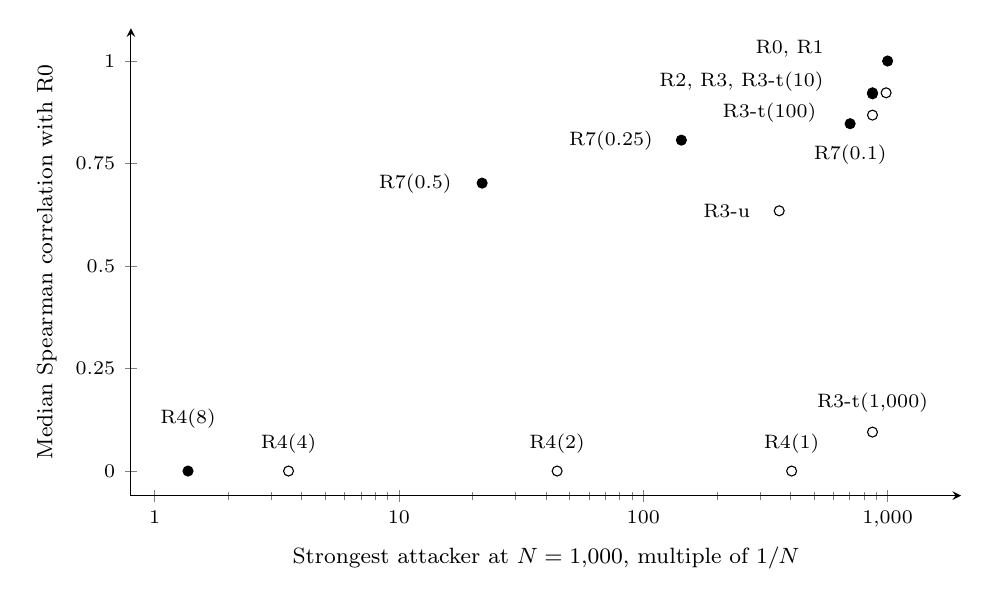
\begin{tikzpicture}
    \begin{semilogxaxis}[
      width=\linewidth, height=0.62\linewidth,
      xmin=0.8, xmax=2000, ymin=-0.06, ymax=1.08,
      xlabel={Strongest attacker at $N = 1{,}000$, multiple of $1/N$},
      ylabel={Median Spearman correlation with R0},
      tick label style={font=\scriptsize}, label style={font=\footnotesize},
      xtick={1,10,100,1000}, xticklabels={1,10,100,1{,}000},
      ytick={0,0.25,0.5,0.75,1}, axis lines=left,
    ]
      % Coordinates from sections/generated/figure-coords.tex. Filled: not dominated; open: dominated.
      \addplot[only marks, mark=*, mark size=1.8pt, black] coordinates
        {(1000,1.0) (867.2,0.9225) (702.4,0.8471) (143.2,0.8070) (21.9,0.7022) (1.37,0.0)};
      \addplot[only marks, mark=o, mark size=1.8pt, black] coordinates
        {(986,0.9225) (867.2,0.9200) (867.2,0.8681) (867.2,0.0950) (360,0.6347) (404.8,0.0) (44.4,0.0) (3.533,0.0)};
      \node[font=\scriptsize, anchor=east] at (axis cs:600,1.03) {R0, R1};
      \node[font=\scriptsize, anchor=east] at (axis cs:600,0.95) {R2, R3, R3-t(10)};
      \node[font=\scriptsize, anchor=east] at (axis cs:560,0.875) {R3-t(100)};
      \node[font=\scriptsize, anchor=north] at (axis cs:702.4,0.82) {R7(0.1)};
      \node[font=\scriptsize, anchor=east] at (axis cs:120,0.807) {R7(0.25)};
      \node[font=\scriptsize, anchor=east] at (axis cs:18,0.702) {R7(0.5)};
      \node[font=\scriptsize, anchor=east] at (axis cs:300,0.635) {R3-u};
      \node[font=\scriptsize, anchor=south] at (axis cs:867.2,0.12) {R3-t(1{,}000)};
      \node[font=\scriptsize, anchor=south] at (axis cs:404.8,0.02) {R4(1)};
      \node[font=\scriptsize, anchor=south] at (axis cs:44.4,0.02) {R4(2)};
      \node[font=\scriptsize, anchor=south] at (axis cs:3.533,0.02) {R4(4)};
      \node[font=\scriptsize, anchor=south] at (axis cs:1.37,0.08) {R4(8)};
    \end{semilogxaxis}
  \end{tikzpicture}
  \caption{No form evaluated brought matching near chance while computing the process measures. Matching against the
  measures for the main forms, full texts, $N = 1{,}000$, attackers with $\lambda = 8$ (lower left: less matching, fewer
  measures); the utility axis has no interval, so dominance by a small difference rests on the point estimates. Filled: forms that no other form dominates, that is, no other form has a lower or equal
  accuracy and a higher or equal correlation, one of them strictly. Open: dominated forms.}
  \label{fig:tradeoff}
\end{figure}

This part asks what each form costs writing research, measured by the agreement of the ten process measures with
their values in R0 (\S\ref{sec:protocol:utility}). R0 and R1 compute all ten measures as before. R2 and R3 compute the
P-bursts, the pauses and the variance of the production rate as in R0 and approximate the R-bursts, deletions and
insertions, with correlations from 0.19 (insertion proportion) to 0.85 (deletion proportion); with the five measures
computed as in R0, the median is 0.92. The approximation rules do not use the position column of R2, so R2 has the
values of R3. At $w = 1{,}000$\,ms five measures cannot be computed,
R3-u loses the pauses within and between words, and R4 computes none (Table~\ref{tab:main}).

Figure~\ref{fig:tradeoff} plots the two axes. The forms that no other form dominates are R0 and R1, R3, the three
levels of suppression and R4(8). R3 dominates R2 and R3-t, which have the same or a lower correlation and the same
accuracy or a higher one, and R7(0.25) dominates R3-u, with a lower accuracy (14.3\% against 36.0\%) and a higher
correlation (0.81 against 0.63). The approximations also change how a
measure relates to the human scores: the mean pause correlates with the score at $-0.11$ in R0 and at $-0.50$ in
R7(0.5), and the R-burst length at $-0.04$ in R0 and at $0.20$ in R2 (Appendix~\ref{app:results}). The utility axis
measures agreement with R0, not whether a measure keeps its relation to the quality of writing.

This is the second axis of contribution C2, read from the forms that no other form dominates. R3 kept 86.7\% with
five measures as in R0 and a median correlation of 0.92; suppressing a tenth, a quarter and a half of the presses gave
70.2\%, 14.3\% and 2.2\% with medians of 0.85, 0.81 and 0.70; R4(8) gave 0.14\% and no measure. Only R4(4) and R4(8)
brought the strongest attacker within four times $1/N$, and they compute no measure; against the exploratory
attackers no form did (\S\ref{sec:results:forms}). Every main form from R2 on computed
the R-burst and insertion measures at a mean correlation below 0.5 or not at all (Appendix~\ref{app:results}).

\subsection{Windows and the open world}
\label{sec:results:windows}

This part asks whether releasing parts of logs changes the picture, and how well the scores separate candidate sets
with and without the true text. On windows, where A1 and A1$'$ are not run, A2 was the strongest attacker on R0 to R3,
R3-t and R4(1), with the same values on all of them, since A2 reads only the segments. At $N = 1{,}000$ it chose the
true window in 65.8\% [63.9, 67.8] of draws with $k = 5$ and in 72.3\% [70.2, 74.5] with $k = 20$; at $N = 10$, in 84\%
to 88\%. On R3-u, where A0 was the strongest attacker, accuracy at $N = 1{,}000$ was 0.6\% to 1.9\%; on R7(0.1), 26.7\%
to 47.5\%; on R4(8), 1.5\% to 16.7\% (Appendix~\ref{app:results}). Each decoy contributed one window, so these values
hold for far fewer candidates than an attacker searching every position of every text would face
(\S\ref{sec:threat-model:bias}), and no process measure is defined on windows.

In the open-world diagnostic, the area was 1.000 for R0 and R1, 0.978 for R2, 0.774 [0.753, 0.795] for R3 and R3-t
and at most 0.62 for the other forms. Within each log, a large margin between the best and the second-best candidate
marked correct matches: on R3, the 80\% of logs and draws with the largest margins were all matched correctly
(exploratory; Appendix~\ref{app:exploratory}). KeyTAR, the reference outside the threat model, stayed
below A0 on every form and $N$ (Appendix~\ref{app:results}).

\subsection{The Japanese translation logs}
\label{sec:results:enja}

This part asks question 4: whether the same kind of matching exceeds chance and A0 on logs typed with an input method,
measured by A2 on R3j at $N$ = all (\S\ref{sec:protocol:enja}). No session met an exclusion criterion, so all 76
sessions of 39 translators on six source texts were used, with 12 or 13 candidates per log. On R3j, which keeps no
string, A2 chose the true translation in 51.6\% [39.3, 63.5] of logs, against $1/N$ = 7.9\% and 11.9\% [5.3, 19.7] for
A0 (means over the six source texts). The differences were 43.7 points [31.4, 55.6] from $1/N$ and 39.7 points [25.6, 53.0] from A0; both lower bounds
are above zero, so by the registered rule matching exceeds chance and A0. Accuracy ranged from 33\% to
77\% over the source texts, and R3j-t($w$) and R4($w$) also exceeded both (Appendix~\ref{app:enja}); A2 reads the same
segments from R3j, R3j-t($w$) and R4(1), so these share its values. The result is
conditional (\S\ref{sec:discussion:limits}): without any string, the categories of input-method events kept enough
of a translation's segment structure to choose it in half of the logs.

\subsection{Exploratory analyses}
\label{sec:results:exploratory}

The exploratory analyses (\S\ref{sec:protocol:exploratory}) are reported in Appendix~\ref{app:exploratory}. Among
them, on R4(2) and R7(0.5) the matches concentrated on 4.2\% and 1.6\% of writers, matched in every draw, and accuracy
differed by score band on R3-u and on several coarse forms.

\section{Discussion and limitations}
\label{sec:discussion}

% Skeleton with draft paragraphs, written before the results. The limitations are written first, from the
% preregistration ("What is not concluded") and Section 3.5; the discussion of the results is added after them.

\subsection{What the results do not show}
\label{sec:discussion:limits}

\paragraph{No proof of safety.}
The results describe the attackers tried here, under the assumptions of Section~\ref{sec:threat-model:bias}. They give
no proof of safety and no upper bound on the risk of matching, and a form that defeats these attackers may not defeat a
stronger one. The strongest attacker is the maximum over the attackers tried, not an attack that combines all the
length and timing information a form leaves; only A3 on R3-u combines the two. The alignment for suppression ignores
the binomial variation and is not a likelihood. The timing term of A3 on R3-u uses, in effect, only the part of a log
before the first error of the replay.

\paragraph{Paths that the forms leave open.}
In the forms that release press times, the duration of a drag, and that of a held key when the next press follows its
release, remains as a lower bound of the next press interval. No attacker targets it, but it can enter the interval
features of A2-b and the segment durations of A3 on R7. The rule that treats the next press after Control as a shortcut
fails when several keys are pressed while Control is held, because whether Control is held cannot be read when its
action time is zero.

\paragraph{The closed world and the candidates.}
The true text is always among the candidates, the attackers always choose one and never abstain, and the open-world
diagnostic does not give a rate of false matches. The decoys are drawn uniformly from the writers of the same prompt,
who may be more or less alike than the members of a class. On windows the attacker knows both ends of the window. The
distribution of accuracy per writer is reported only up to its 90th percentile.

\paragraph{What the data allow.}
We claim no difference by writer attributes, since the demographic file was not acquired, and we do not describe matching
as identification of writers. The results on KLiCKe are not generalised to other tasks (a limit of 30 minutes,
argumentative essays, crowdsourced writers) or to logs that did not pass the selection of the KLiCKe release, such as
logs with much pasting~\cite{tian2025klicke}. The results on ENJA15 are not generalised to Japanese free writing or to
logs of input methods in general, and differences from KLiCKe are not attributed to language or input method, since
the task, the input and the language differ at once. Our formulas for the process measures could not be verified
against Inputlog (\S\ref{sec:protocol:utility}). KeyTAR was run with the defaults of its artifact, including a limit on
generated tokens that is expected to cut reconstructions short, and is a reference, not a bound.

\paragraph{The exploratory analyses.}
The uniqueness of word-length sequences is measured among the $N$ candidates tried and is not a risk of
re-identification in a population. The form with differentially private noise gives its guarantee for one segment
count or one interval, not for a writer's log, and its noise comes from a seeded generator for evaluation, not from an
implementation suitable for release.

\subsection{Processing and agreements}
\label{sec:discussion:agreements}

Processing is not the only protection that a releasing party can give. A release can also be bound by terms of
use. The terms of DataShop, a repository of data from educational software, state ``You will not make any attempts to
de-anonymize the data'' and forbid creating a dataset with information that identifies
students~\cite{datashop2012terms}. The rules of the competition allow the data to be used for non-commercial purposes,
including academic research, and forbid passing them to anyone who has not agreed to the rules; in the rules and on the
data page we found no clause on recovering the texts or identifying the writers~\cite{kaggle2023lwp}. KLiCKe may be
downloaded and used freely, with the repository cited as the source~\cite{inputlog2026community}. Terms do not change
what a log reveals to a party that ignores them, and they do not bind a party that holds the texts and obtains the
logs outside the terms; but they define who may use a release and for what, and they can be combined with any of the
forms evaluated here.

\subsection{What a releasing party can take away}
\label{sec:discussion:takeaways}

\textbf{[After the results.]} The results are material for three choices: which columns to keep, how coarsely to give
times and lengths, and whether to release full logs or windows. Each statement takes the form ``against this attacker,
at this $N$, this form had this multiple of $1/N$ and kept this much of the process measures''. No rule recommends a
form, and the paper does not say that a form works or withstands matching.

\section{Conclusion}
\label{sec:conclusion}

We asked how far each form of processing keeps a keystroke log apart from its text against a party that holds
candidate texts, and what each form costs the process measures of writing research. Against attackers that know the
processing, the masking used in one public release, applied to a public corpus of the same kind, left every essay
matched among 1,000 candidates. Among the forms that release less, matching fell only with the process measures:
halving the presses left 2.2\%, no more than the total length alone gave, with a median correlation of 0.70, and only
forms that compute no measure came closer to chance; stronger attackers tried afterwards as an exploration matched more
on most coarse forms. Hiding the characters in this way did not keep the logs apart from texts held elsewhere. These are
measurements of the attackers and corpora tried, not bounds on the risk.


% Only in the preprint: the submission is anonymous (main.tex keeps "To be written for the camera-ready version").
\section*{Acknowledgements}
We thank Yu Tian for answering our questions about the KLiCKe corpus and for reading a draft of this paper, and the
authors of the KLiCKe corpus for releasing it.

\begin{ethics}
To be written.
\end{ethics}

\begin{openscience}
To be written.
\end{openscience}

\begin{ai}
To be written.
\end{ai}


\bibliographystyle{abbrvnat}
\bibliography{references}

\appendix
\section{Checks after acquisition and on synthetic logs}
\label{app:checks}

% Moved from Sections 4.2, 4.3 and 5.1 of the main body on 24 October 2026, without changing the procedure. The text
% is that of the main body before the move, except for the references back to it.

\subsection{Checks after acquisition}
\label{sec:data:checks}

Before any value of matching or utility was computed, the preregistration allowed only a fixed list of checks: the
counts of files, rows, writers and excluded writers; the column names and values; the share of logs whose final draft,
rebuilt from the unprocessed log, matches the distributed text; the error of the segment rule
(\S\ref{sec:attackers:segments}); the structure of ENJA15; the inference time of KeyTAR on one log; and a verification
of our formulas for the process measures. The checks report counts only; the scripts print no writer identifier, no
text and no log.

\paragraph{Escaped characters.}
The distributed logs write four characters (newline, tab, double quote and backslash) in the text change and key
columns as two-character escape sequences, which the procedure did not anticipate. Read as they are, a newline is
inserted as two characters and the rebuilt draft drifts from the cursor position. We undo the escapes when the logs are
read and change nothing else in the procedure; this is reported as a deviation, with the values of the checks before
and after the change. After it, the final draft rebuilt from the unprocessed log matches the distributed text exactly,
after normalisation of whitespace, for 4,842 of the 4,992 writers (97.0\%), against 72 before. The other 150 writers
stay in full-text matching, and accuracy is also reported separately for writers whose rebuilt draft matches and
writers whose draft does not.

\paragraph{Other checks.}
The action time of modifier keys, which the corpus description gives as zero~\cite{tian2025klicke}, is zero for Shift,
Control and Alt but not for most CapsLock and Meta presses. No attacker uses hold times and the coarser forms drop
them, so the procedure is unchanged. The corpus does not distribute the process measures computed by Inputlog, so the
verification of our formulas against them could not be done (\S\ref{sec:protocol:utility}). For KeyTAR, the default
settings of the artifact were recorded, and the inference on one log fitted in the memory of a 16\,GB GPU.

\paragraph{Cases that the segment rule misses.}
The rule ``the next press after Control'' misses shortcuts made with several keys while Control is held,
such as two successive undos, and pastes made from a menu: in 566 of the 1,133 paste events of the corpus, the
preceding press, ignoring Shift, Alt and CapsLock, is not Control.

\subsection{A check on synthetic logs before registration}
\label{app:checks:synthetic}

Before the preregistration was fixed, we checked on synthetic logs, with no human data, whether the lengths of words
can be recovered from columns other than the key categories. The synthetic logs included deletion, deletion of a
selection, replacement, paste, cursor movement by arrows, Home, End and mouse, and undo. In pairs of synthetic logs
that share the category sequence and the press times and differ only in hidden choices, such as the target of a mouse
click or the pasted words, forms R3, R3-u, R3-t and R7 gave identical output, while R0, R1 and R2 differed in every
pair (R2 through the position and the word count). The release times were at first kept in these forms; in a
simulation in which a drag's duration appears in its hold time, the output differed through them, and they were then
dropped. A drag's duration, and that of a held key when the next press follows its release, still remains as a lower
bound of the next press interval, which a form that releases press times cannot remove. In R2, rebuilding the draft
from the cursor position recovered the exact sequence of word lengths in 64\% of the synthetic logs with light
editing. These checks led to the present definitions of the forms, the categories and the segment rule, which are part
of the registered plan.

\section{Methods for the Japanese translation logs}
\label{app:enja}

% Moved from Sections 4.1, 4.3, 5.5 and 6.6 of the main body on 24 October 2026, without changing the procedure. The
% main body keeps the candidates, the segment rule, the quantity that answers question 4 and the rule for "exceeds".

\paragraph{Corpus.}
ENJA15 is a public corpus of English-to-Japanese translation processes recorded with Translog-II, in which Japanese was
typed with an input method~\cite{carl2016lrec,zou2026translog}. We use only the from-scratch translation sessions and
take the final translation recorded in each log as its text. The sessions were acquired on 12 October 2026 (UTC) from
the repository of the database that distributes them, at a fixed revision. The database states two licences on two of
its pages; both are non-commercial with attribution, and we follow the more restrictive one, which also requires
derived works to be shared alike~\cite{crittlicense}. The corpus has 76 from-scratch sessions by 39 translators on six
source texts, with 12 or 13 translators per source text. Thirty-seven translators translated two source texts and two
translated one, so translators and source texts are crossed. Sessions are excluded if the log or translation is missing,
if the translation is empty, or if the log contains neither an input-method event nor an inserted letter.

\paragraph{Forms.}
For ENJA15 the forms are R0j (no processing); R3j, which keeps the event type and the time and replaces each key event
by one of the categories romaji letter, conversion, commit, commit containing punctuation, BackSpace, Enter, navigation
and other, and removes every string (the key name, the committed text and the keys typed for it); R3j-t($w$), with the
press times of R3j rounded ($w = 10$, $100$, $1{,}000$\,ms); and R4($w$). The logs have no release events, so hold
times do not arise. Before the main computation we checked on all sessions, which include updates of uncommitted
strings, conversions, cancelled conversions and commits, that no row of R3j keeps a string of its session.

\paragraph{Attackers.}
In a translation, segments are split at the Japanese comma and full stop (U+3001, U+3002, U+FF0C and U+FF0E) and at
line breaks, and the value of a segment
is the standard number of keystrokes needed to type its reading with an input method, from the readings of a
morphological analyser and a romaji conversion table. In a log, among the input-method and insertion events, a letter
press adds 1, a BackSpace press subtracts 1, and a commit that contains punctuation closes the segment. Only A0 and A2
are run on these logs. A1, A1$'$, A3 and A4 are not, because they rely on rebuilding the final draft or on models of
English. A0 compares the number of letter presses minus BackSpace presses with the sum of the keystroke counts of the
candidate's readings. A2 aligns the segments as on KLiCKe, with the same groups and $\lambda$. Neither reads a string,
so they give the same values on R0j, R3j and R3j-t; in R0j the committed strings remain in the log and matching is
trivial for an attacker that reads them, so R0j is only a reference.

\paragraph{Analysis.}
The fourth question of the study asks how far above chance and above A0 the same kind of matching is on the Japanese
translation logs. The candidates for a log are translations of the same source text by other translators: all of them
($N$ = all), or nine drawn without replacement, 20 times per log ($N = 10$); identical translations tie. Accuracy, $1/N$
and the accuracy of A0 are averaged over the logs of each source text and then over the source texts. Since
translators and source texts are crossed, intervals come from 2,000 bootstrap resamples of translators with all their
sessions, without stratification, and differences are taken within each resample. The quantity that answers the
question is the accuracy of A2 on R3j, full texts and $N$ = all, with its differences from $1/N$ and from A0. We say
that matching ``exceeds'' chance and A0 only if the lower bounds of the intervals of both differences are above zero.
R3j-t($w$) and R4($w$) are reported with the same rule; since neither A0 nor A2 uses times, R3j-t($w$) gives the
values of R3j. Values per source text are only described, and R0j is a reference. ENJA15 is much smaller than KLiCKe, and its intervals are expected to be wide.

\section{Details of the attackers and of windows}
\label{app:attackers}

% Moved from Sections 4.1, 5.3, 5.4, 6.1 and 6.5 of the main body on 24 October 2026, without changing the
% procedure.

\paragraph{The KeyTAR model.}
KeyTAR reconstructs typed text from keystroke intervals with a fine-tuned language model~\cite{qiu2026keytar}. We use
its public artifact as released (Zenodo record 17254163), with the checkpoint trained on intervals recorded from typing
rather than on intervals recovered through a cache side channel. The artifact is released under the MIT License and the
record under CC~BY~4.0; its statements on ethics and intended use do not exclude reconstruction from the intervals of
public keystroke data. We do not fine-tune it on KLiCKe, and it runs on a local GPU.

\paragraph{A4: KeyTAR.}
A4 takes the intervals between letter, digit and space presses, cuts them into chunks of 20 record segments, gives
each chunk to the public KeyTAR model to reconstruct the text, and chooses the candidate with the smallest normalised
edit distance to the concatenated reconstruction, after both are lowercased and every character other than a letter or
digit is replaced by a space. The model is used with the default settings of its artifact, with intervals capped at
1,023\,ms as in its training data and without preceding context. Among the defaults is a limit of 50 generated tokens
per chunk, which is expected to cut the reconstruction of many chunks short; we kept it as registered rather than
choose, after the fact, a setting that would make the attacker stronger. KeyTAR assumes ordinary English input without
revision~\cite{qiu2026keytar}, it contains a language model, and it does not adapt to the processing. It is therefore
reported in a separate row and is not part of the strongest attacker. The intervals it uses are the same in R0, R1,
R2 and R3, so these forms share one reconstruction.

\paragraph{Alignment and A3.}
Among alignment paths of equal cost, the group listed first is chosen, and where the end can be chosen, the earlier
position in the text. A3 estimates the mean and variance of the logarithm of the press interval for each pair of
consecutive characters; a pair seen fewer than 20 times takes the values of its pair of character types (such as
letter followed by space), and a type pair seen fewer than 20 times takes the values of all intervals. In R3-u the
A1$'$ replay gives the sequence of ``char'' items of the final draft, matched one to one from the start with all
characters of the candidate; the timing term uses the intervals between adjacent final characters that were typed
consecutively, and the length term is the log-likelihood of the difference between the replayed count and the
candidate's character count, estimated on the training logs. The timing term is used both as a sum and as a mean per
term, and the better version is reported as A3 on R3-u; a version with the length term alone separates the
contribution of timing. The check on synthetic logs showed that the one-to-one correspondence in R3-u uses in effect
only the part of the log before the first replay error. In R7, A3 scores the duration of each segment, from its first
to its last remaining press, with a regression on the logarithm of the candidate segment's character count, estimated
on training logs with the same suppression. Details that the registration left open, such as how an interval is
scored when the candidate word has fewer characters than the segment has intervals, were fixed on synthetic logs
before the data were opened and are documented with the code.

\paragraph{The attackers on windows.}
On windows, A0 counts the window's presses as on full texts and compares the count with the candidate window. A1 and
A1$'$ are not run, since a part of the process does not determine the final draft. A2 and A2-b align the window's
segments with the candidate window, with the window end of the alignment; A2 is also run on R0, R1, R5 and R6, whose
key categories allow segments to be built. A3 uses the A2 alignment (in R3-u the A2-b alignment, and the timing term
alone, since the length term is the count of A0). On full texts A3 on R3-u uses the one-to-one correspondence of the
replay, so its difference between full texts and windows also reflects the change of mechanism. A4 reconstructs the
window's intervals and compares the reconstruction with the candidate window.

\paragraph{Candidate windows.}
Windows contain $k = 5$, $10$, $20$ or $50$ non-empty segments (\S\ref{sec:attackers:windows}), with five window starts
per log drawn uniformly from the valid starts. The true window is found once, on the unprocessed log, and used by
every form and attacker. Replaying the log gives, for each press, the character of the final draft that it became; the
true window is the $k$ words of the text that start at the word holding most of the surviving characters of the
window's first segment. Windows whose first segment leaves no character in the final draft, and windows that would run
past the end of the text, are not used. For writers whose rebuilt draft does not match the distributed text, the words
of the two are aligned after normalisation of whitespace, and only windows whose first word maps to a word of the
distributed text are used; the windows that do not map are counted. Each decoy contributes one window of $k$ words,
drawn uniformly from its valid windows. Logs with no valid window of length $k$ are left out for that $k$, and their
number is reported.

\paragraph{Position of true windows.}
To see whether true windows sit at positions that favour the alignment, we show the distribution of the A2 alignment
cost at the true window next to that of the whole log.

\section{Exploratory analyses: procedures}
\label{app:exploratory}

% Moved from Section 6.7 of the main body on 24 October 2026. The text of the procedures is unchanged; the tables are
% added after the main computation (24 October 2026); they are generated by make_tables.py.

% The record of the main computation (notes.md) confirms that no value of matching or utility had been opened before
% the procedures of the last three analyses were committed; the main results were first written on 24 October 2026.
% Analyses 6 and 7 were decided on 29 October 2026, after the main results; their
% procedures are in notes.md ("procedures, part 3"), committed that day, and they ran from 12 to 17 November 2026.
Seven analyses were added after the preregistration was fixed and are not part of it. They change no registered value
or procedure, are reported as exploratory and are not used to answer the four questions. The procedures of the first
five were fixed and committed to the study repository before any value of matching or utility on the human data had
been seen, the first two on 13 October 2026 and the other three on 21 October 2026, as the record of that repository
shows. The third to fifth use the strongest
attacker selected in the main computation for the same form and $N$, without selecting again, on full texts, the main
forms, $N = 10$ and $1{,}000$ and the 500 writers, with the same resamples. The last two were decided after the main
results had been seen, because the full-text accuracy on the coarse forms was far below that on windows and with the
lighter penalty (\S\ref{sec:results:forms}); their procedures were committed on 29 October 2026, before they were
run. They aim to strengthen the attackers, not to protect a form.

\paragraph{Uniqueness of word-length sequences among $N$ candidates.}
The first analysis uses the texts alone. For each of the 500 writers and each $k$ from 1 to 50, five runs of $k$
consecutive words are drawn from the writer's text, and we report the share for which none of the $N - 1$ decoys,
drawn as in the main computation, contains the same sequence of word lengths at any position; as a secondary quantity,
the accuracy $1/m$ of an attacker who chooses uniformly among the $m$ texts that contain it. Next to these curves we
draw reference lines $k^{*} = \log_2 N / h$, where $h$ is a plug-in estimate of the entropy rate of word lengths in
bits per word, conditioned on up to two preceding words~\cite{kalimeri2012entropy}; plug-in estimates fall as the
order rises, and the lines are a reference, not a prediction. We call the quantity uniqueness among $N$ candidates and
not a risk of re-identification. Whether uniqueness in a sample says anything about a population is
disputed~\cite{sanchez2016comment,rocher2019estimating}, and in location data unicity decreases, slowly, as the dataset
grows~\cite{farzanehfar2021risk}; here the population is the set of $N$ candidates itself, and we do not extend the
quantity beyond the values of $N$ tried.

\paragraph{A form with differentially private noise.}
The second analysis adds a form R-DP($\varepsilon$), $\varepsilon = 0.5$, $1$, $2$, $4$, built on R3, with letters and
digits released as one category. Two mechanisms use the same $\varepsilon$. First, the number of counted letter and
digit presses of each segment receives two-sided geometric noise with sensitivity 1, and letter presses are added at
random positions in the segment or removed at random accordingly, with the count kept at zero or above. Second, every
press interval is clipped at 2,000\,ms, the threshold of the P-bursts, and receives two-sided geometric noise with
sensitivity 2,000\,ms, and negative intervals are set to zero. Each guarantee holds for its own unit, one segment count
or one interval, and not for a writer's whole log: over a log the budgets add up over all segments and
intervals~\cite{kellaris2014event}. We do not claim that the combined release is differentially private for neighbouring
logs that differ by an inserted or removed press with its time. The noise is drawn from a seeded generator so that the
evaluation can be repeated, which is acceptable for evaluation but not for an actual release~\cite{holohan2023random},
and an actual release would also need an implementation that is exact on finite
computers~\cite{canonne2020discrete}. The attackers are those of R3, with the timing table of A3 built from training
logs with the same interval noise; the candidates are unchanged, and every process measure that R3 computes is counted as
approximated. The scope, samples and resamples are those of the main computation, with the contrast R3~$-$~R-DP and the
open-world area, but no negative control. R-DP is reported in exploratory tables, where $\varepsilon$ is labelled as the budget per segment count and per
interval, and it is not part of the main table or figure.

\paragraph{The upper tail of accuracy per writer.}
The third analysis reports the 95th and 99th percentiles of accuracy per writer and the share of writers whose true text
is chosen alone in every draw. No value per writer is reported.

\paragraph{Matches above a margin.}
The fourth analysis takes, for each log and draw, the difference between the attacker's second-lowest and lowest cost
over the candidates (zero if the lowest is tied), with log-likelihoods turned into costs by a change of sign. At
thresholds set at the 0th, 10th, \ldots, 90th percentiles of these differences, it reports the share of logs and draws
at or above the threshold and the accuracy among them. Costs of different attackers are not compared.

\paragraph{Accuracy by score band.}
The fifth analysis divides the 125 sampled writers of each prompt into thirds by their human score and reports the strongest
attacker's accuracy in each third and the difference between the top and bottom thirds. The attackers do not use the
scores.

\paragraph{A grid of the penalty.}
The sixth analysis runs A2 on R3, R4($w$) and R7($p$), and A1$'$ on R3 and R7($p$), the forms on which the main
computation runs it, with $\lambda = 2$, $4$, $8$ and $16$ in the alignment of \S\ref{sec:attackers:alignment}, which is
otherwise unchanged. The main computation left R7 out of the registered secondary analysis with $\lambda = 4$ and 16 (a deviation,
Appendix~\ref{app:checks:deviations}), so the values of R7 with $\lambda = 4$ and 16 are those of that analysis,
computed here after the main results, and those with $\lambda = 2$ are new. As positive controls, A2 and A1$'$ with $\lambda = 8$ equal the cells of the main
computation at both $N$, and A2 with $\lambda = 4$ and $16$ equals the secondary analysis on R3 and R4($w$) at
$N = 1{,}000$.

\paragraph{A full-text attacker that aligns chunks.}
The seventh analysis, A2-scan, cuts the record values of A2 into consecutive chunks of 20 segments from the start of
the log and drops a last chunk of fewer than five segments; a log with no chunk leaves all candidates tied. Each chunk
is aligned with the word lengths of a candidate, starting and ending anywhere in the text, with the groups and the
penalty of A2. A candidate's cost is the sum of the costs of the chunks, infinite if a chunk has no path, and the
candidate with the lowest cost is chosen. For simplicity, chunks may overlap or change order within a candidate. It
runs with $\lambda = 2$, $4$, $8$ and $16$ on the forms of the sixth analysis. As controls on synthetic writers, one
chunk holding the whole log reproduces the costs of A2 on windows when its start is fixed and on full texts when both
ends are fixed.

\paragraph{The strongest attacker with the variants.}
For each form and $N$, the strongest attacker with the variants is the maximum over the attackers of the main
computation and the variants of the sixth and seventh analyses, selected again in every resample. Selecting on the
evaluated logs favours the attacker (\S\ref{sec:threat-model:bias}). Thirteen of the fourteen pairs of form and $N$
that a variant won were won with $\lambda = 2$, the lowest value of the grid, and the other with $\lambda = 16$
(Table~\ref{tab:app:stronger}); a lighter penalty might match more, and was not tried. The process measures do not
change, since the forms do not.

\paragraph{Tables.}
% The computation of R-DP (run_main.py --forms dp) ran R3 and R-DP without R0, so the summaries of the process measures
% relative to R0 were empty in exploratory_dp.json (notes.md, D5). They were recomputed from the caches with R0 of the
% main computation, with the same sample and resamples (exploratory_dp_utility_r0.json); the values of R3 equal those
% of main.json.
Tables~\ref{tab:app:unicity} to~\ref{tab:app:band} give the first five analyses, and
Tables~\ref{tab:app:lambda-1000} to~\ref{tab:app:stronger} the last two.

\begin{table*}
  \caption{Exploratory: uniqueness of word-length sequences among $N$ candidates, 500 writers. Unique: the percentage
  of runs of $k$ consecutive words whose sequence of word lengths no decoy contains, averaged per writer and then over
  writers, with its interval. $1/m$: the accuracy of choosing uniformly among the $m$ candidates that contain the
  sequence. All: unique at $N = 1{,}000$ for all writers after exclusion. $k^{*}$: the reference lines $\log_2 N / h_j$ for
  $j = 0$, $1$, $2$ preceding words, with $h_j$ the plug-in entropy rate of word lengths over all writers after exclusion.}
  \label{tab:app:unicity}
  \small
  \begin{tabular}{rllllllr}
    \toprule
    & \multicolumn{2}{l}{$N = 10$} & \multicolumn{2}{l}{$N = 100$} & \multicolumn{2}{l}{$N = 1{,}000$} & All \\
    $k$ & Unique & $1/m$ & Unique & $1/m$ & Unique & $1/m$ & $1{,}000$ \\
    \midrule
    \tabinput{sections/generated/explore-unicity.tex}
    \bottomrule
  \end{tabular}
\end{table*}

\begin{table*}
  \caption{Exploratory: R-DP($\varepsilon$), with $\varepsilon$ the budget per segment count and per interval, not per
  writer, and R3, 500 writers. Full texts: the accuracy of the strongest attacker, A1$'$ on every form and $N$, and the
  contrast R3~$-$~R-DP in points at $N = 1{,}000$. Windows: the accuracy of the strongest attacker, A2, at
  $N = 1{,}000$. Area: the open-world area. The values of R3 are those of the main computation.}
  \label{tab:app:dp}
  \small
  \begin{tabular}{lrrlllllll}
    \toprule
    & \multicolumn{4}{l}{Full texts} & \multicolumn{4}{l}{Windows, $N = 1{,}000$} & \\
    Form & $N = 10$ & $100$ & $1{,}000$ & R3~$-$~form & $k = 5$ & $10$ & $20$ & $50$ & Area \\
    \midrule
    \tabinput{sections/generated/explore-dp.tex}
    \bottomrule
  \end{tabular}
\end{table*}

\begin{table*}
  \caption{Exploratory: process measures on R3 and R-DP($\varepsilon$), 500 writers, mean over the four prompts. Top:
  the Spearman correlation with the value in R0. Bottom: the Spearman correlation with the human score. Every measure
  on R-DP is approximated.}
  \label{tab:app:dp-score}
  \small
  \begin{tabular}{lrrrrr}
    \toprule
    Measure & R3 & R-DP(4) & R-DP(2) & R-DP(1) & R-DP(0.5) \\
    \midrule
    \multicolumn{6}{l}{Correlation with R0} \\
    \tabinput{sections/generated/explore-dp-r0.tex}
    \midrule
    \multicolumn{6}{l}{Correlation with the human score} \\
    \tabinput{sections/generated/explore-dp-score.tex}
    \bottomrule
  \end{tabular}
\end{table*}

\begin{table*}
  \caption{Exploratory: the upper tail of accuracy per writer, full texts, 500 writers: the 95th and 99th percentiles
  and the share of writers whose true text was chosen alone in every draw.}
  \label{tab:app:tail}
  \small
    \begin{tabular}{lrllll}
    \toprule
    Form & $N$ & Attacker & 95th & 99th & Every draw \\
    \midrule
    \tabinput{sections/generated/explore-tail.tex}
    \bottomrule
  \end{tabular}
\end{table*}

\begin{table*}
  \caption{Exploratory: matches above a margin, full texts, 500 writers. For thresholds at the 0th, 20th, 50th, 80th
  and 90th percentiles of the margin between the second-lowest and the lowest cost, the share of logs and draws at or
  above the threshold and the accuracy among them (share/accuracy). Costs of different attackers are not comparable.}
  \label{tab:app:margin}
  \small
  \begin{tabular}{lrllllll}
    \toprule
    Form & $N$ & Attacker & 0th & 20th & 50th & 80th & 90th \\
    \midrule
    \tabinput{sections/generated/explore-margin.tex}
    \bottomrule
  \end{tabular}
\end{table*}

\begin{table*}
  \caption{Exploratory: accuracy by score band (thirds of each prompt's sampled writers, lowest first), full texts,
  and the difference between the highest and the lowest third.}
  \label{tab:app:band}
  \small
    \begin{tabular}{lrlrrrl}
    \toprule
    Form & $N$ & Att. & Low & Mid & High & High $-$ low \\
    \midrule
    \tabinput{sections/generated/explore-band.tex}
    \bottomrule
  \end{tabular}
\end{table*}

\begin{table*}
  \caption{Exploratory: accuracy (\%) of every variant of the sixth and seventh analyses, full texts, $N = 1{,}000$, with
  intervals. A2 and A1$'$ with $\lambda = 8$ are the attackers of the main computation; A2-scan aligns chunks of 20
  segments anywhere in the text.}
  \label{tab:app:lambda-1000}
  \small
  \begin{tabular}{llllll}
    \toprule
    Form & Attacker & $\lambda = 2$ & $\lambda = 4$ & $\lambda = 8$ & $\lambda = 16$ \\
    \midrule
    \tabinput{sections/generated/explore-lambda-scan-1000.tex}
    \bottomrule
  \end{tabular}
\end{table*}

\begin{table*}
  \caption{Exploratory: accuracy (\%) of every variant of the sixth and seventh analyses, full texts, $N = 10$, with
  intervals. A2 and A1$'$ with $\lambda = 8$ are the attackers of the main computation; A2-scan aligns chunks of 20
  segments anywhere in the text.}
  \label{tab:app:lambda-10}
  \small
  \begin{tabular}{llllll}
    \toprule
    Form & Attacker & $\lambda = 2$ & $\lambda = 4$ & $\lambda = 8$ & $\lambda = 16$ \\
    \midrule
    \tabinput{sections/generated/explore-lambda-scan-10.tex}
    \bottomrule
  \end{tabular}
\end{table*}

\begin{table*}
  \caption{Exploratory: the strongest attacker of the main computation (Main) and the strongest attacker with the
  variants of the sixth and seventh analyses (With variants, selected again in every resample, with its interval and
  the attacker chosen, with the percentage of resamples in parentheses when below 100), full texts, accuracy in
  percent. Difference: with variants minus main at $N = 1{,}000$, with its interval.}
  \label{tab:app:stronger}
  \small
  \begin{tabular}{lllllllr}
    \toprule
    & \multicolumn{3}{l}{$N = 10$} & \multicolumn{4}{l}{$N = 1{,}000$} \\
    Form & Main & With variants & Attacker & Main & With variants & Attacker & Difference \\
    \midrule
    \tabinput{sections/generated/explore-strongest.tex}
    \bottomrule
  \end{tabular}
\end{table*}

\section{Forms R5 and R6, secondary quantities and results for all writers}
\label{app:results}

% The definitions of R5 and R6 and the list of secondary quantities were moved from Sections 4.3 and 6.2 of the main
% body on 24 October 2026, without changing the procedure. The tables are added after the main computation.

\paragraph{Forms R5 and R6.}
R5 (substitution) and R6 (permutation) are our definitions after the names of processing steps in Vassallo et
al.~\cite{vassallo2017privacy}, whose full text we could not obtain; they do not reproduce that work. Their columns,
in the terms of Table~\ref{tab:forms}, are:
\begin{itemize}
  \item R5 Substitution. Pressed key: letters and digits to a random neighbour on a QWERTY keyboard. Activity and text
    change: as is, with the same substitution. Position and word count: as is. Times: as is.
  \item R6 Permutation. Pressed key: typed letters and digits permuted within each segment. Activity and text change:
    as is, with the same permutation; letters and digits of pasted, replaced and removed strings to \texttt{q}.
    Position and word count: as is. Times: as is.
\end{itemize}

\paragraph{Secondary quantities.}
We also report the rank of the true text (top-5 accuracy and mean reciprocal rank); the distribution of accuracy per
writer, at its 10th, 50th and 90th percentiles; A2 with $\lambda = 4$ and $16$ ($N = 1{,}000$, full text); accuracy
separately for writers whose rebuilt draft matches the distributed text and writers whose draft does not; and the
numbers of candidates without an alignment path.

\paragraph{Results.}
\textbf{[After the main computation: every cell of the main computation, including attackers A0 to A3 on all writers
after exclusion, forms R5 and R6, the full rows of KeyTAR and the secondary quantities.]}


\end{document}
